% p10-05 例 1：矩形 AB=6 BC=8，沿 BE 折 △ABE 使 A 落到 BC 上 A'。求 AE.
% 文中坐标 A(0,0), B(6,0), C(6,8), D(0,8)；A' ∈ BC，BA'=6 → A'=(6,6)；AE=6 → E=(0,6)
\documentclass[tikz,border=4pt]{standalone}
\usepackage{ctex}
\usepackage{amsmath}
\usetikzlibrary{calc}
\begin{document}
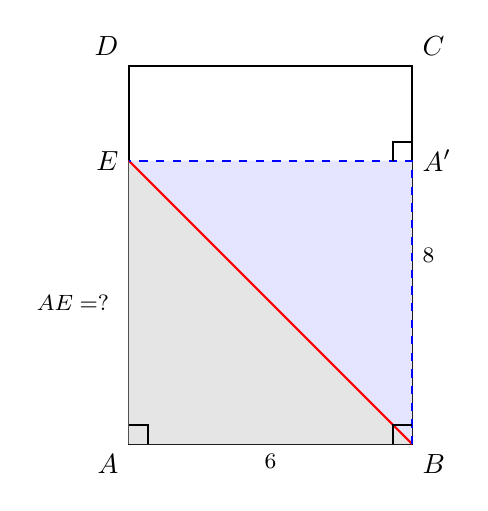
\begin{tikzpicture}[scale=0.6, thick]
  \coordinate (A) at (0,0);
  \coordinate (B) at (6,0);
  \coordinate (C) at (6,8);
  \coordinate (D) at (0,8);
  \coordinate (E) at (0,6);   % AE = 6
  \coordinate (Ap) at (6,6);  % BA' = 6, on BC

  \draw (A)--(B)--(C)--(D)--cycle;

  % 折前 △ABE（灰填充）
  \fill[black!10] (A)--(B)--(E)--cycle;
  % 折后 △A'BE（蓝虚线）
  \fill[blue!10] (Ap)--(B)--(E)--cycle;

  \draw[red, thick] (B)--(E);                % 折痕
  \draw[blue, dashed, thick] (B)--(Ap)--(E);

  % 直角符号
  \draw ($(A)+(0.4,0)$)--($(A)+(0.4,0.4)$)--($(A)+(0,0.4)$);
  \draw ($(B)+(-0.4,0)$)--($(B)+(-0.4,0.4)$)--($(B)+(0,0.4)$);
  % ∠BA'E = 90°
  \draw ($(Ap)+(-0.4,0)$)--($(Ap)+(-0.4,0.4)$)--($(Ap)+(0,0.4)$);

  \node[below left]  at (A) {$A$};
  \node[below right] at (B) {$B$};
  \node[above right] at (C) {$C$};
  \node[above left]  at (D) {$D$};
  \node[left]  at (E) {$E$};
  \node[right] at (Ap) {$A'$};

  \node[below] at ($(A)!0.5!(B)$) {\footnotesize $6$};
  \node[right] at ($(B)!0.5!(C)$) {\footnotesize $8$};
  \node[left, font=\footnotesize] at (-0.2, 3) {$AE=?$};
\end{tikzpicture}
\end{document}
